\chapter{High gain one stage OTA}

\begin{wrapfigure}{l}{0pt}
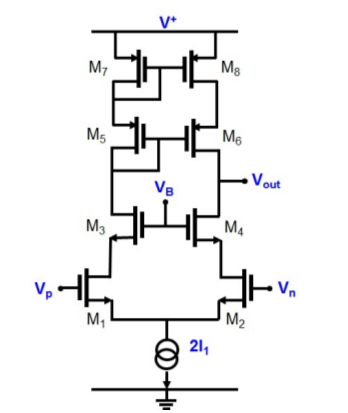
\includegraphics[width=0.25\textwidth]{telescopiccascode.png}
\end{wrapfigure}

\section{Telescopic cascode}
\subsection{Gain}
Considering all transistors with the same $r_0$
\begin{equation}
G_d=\frac{(g_{m1}r_0)^2}{2}
\end{equation}
If the $r_0$ are different we get
\begin{equation}
r_{down}=\frac{r_{04}+2r_{02}+2g_{m4}r_{04}r_{02}}{2}\simeq \frac{2g_{m4}r_{04}r_{02}}{2}=g_{m4}r_{04}r_{02}
\end{equation}
\begin{equation}
r_{up}=r_{06}+r_{08}+g_{m6}r_{06}r_{08}\simeq g_{m6}r_{06}r_{08}
\end{equation}
so for Norton theorem
\begin{equation}
G_d=g_{m1}\cdot r_{down}//r_{up}
\end{equation}


\subsection{Dynamics}

{\bf Output voltage swing}\\
Upper voltage limited by M6 saturation 
\begin{equation}
V_{out}^{max}=V_{dd}-V_{gs8}+V_{ov6}
\end{equation}
Lower voltage limited by M4 saturation
\begin{equation}
V_{out}^{min}=V_B-V_t
\end{equation}
{\bf Input common mode range}\\
Upper voltage limited by saturation of M1-M2
\begin{equation}
V_{CM}^{max}=V_B-V_{gs4}+V_t
\end{equation}
Lower voltage limited by saturation of the tail current generator
\begin{equation}
V_{CM}^{min}=V_{ovG}+V_{gs1}
\end{equation}

The setting of $V_B$ is quite critical. By decreasing $V_B$ , the output swing
increases, but reducing the common-mode swing.\\
\begin{equation}
V_B^{max}=V_{dd}-V_{gs7}-V_{ov6}\ \ \ \ \ V_B^{min}=V_{ovG}+V_{ov2}+V_{gs3}
\end{equation}

%------------------------------------------------------------------------%
\section{Folded cascode}
%------------------------------------------------------------------------%
\centering
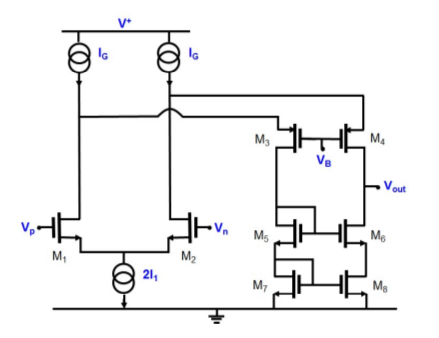
\includegraphics[width=0.6\textwidth]{foldedcascode.png}\\
\raggedright

\begin{wrapfigure}{i}{0pt}
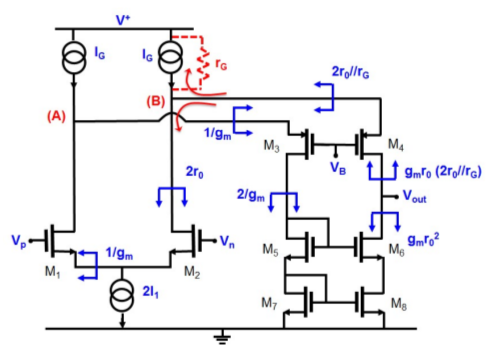
\includegraphics[width=0.5\textwidth]{foldedcascoderes.png}
\end{wrapfigure}

\subsection{Gain}
Using Norton theorem
\begin{equation}
r_{down}=r_{06}+r_{08}+g_{m6}r_{06}r_{08}\simeq g_{m6}r_{06}r_{08}
\end{equation}
The upper resistance without taking into account the loop is 
\begin{equation}
r_{up}^{no-loop}=r_{04}+r_{0g}//2r_{02}+g_{m4}r_{04}(r_{0g}//2r_{02}\simeq g_{m4}r_{04}(r_{0g}//2r_{02})
\end{equation}
The $G_{loop}$ is now 
\begin{equation}
G_{loop}=-\frac{r_{0g}}{r_{0g}+2r_{02}}
\end{equation}
Therefore we have 
\begin{equation}
r_{up}\simeq g_{m4}r_{04}(r_{04}//r_{0g})
\end{equation}
and a differential gain of 
\begin{equation}
G_d=g_{m1}g_{m4}\cdot r_{up}//r_{down}\simeq \frac{(g_mr_0)^2}{3}
\end{equation}

\subsection{n-mos dynamics}

{\bf Output voltage swing}\\
Upper voltage limited by the saturation of M4
\begin{equation}
V_{out}^{max}=V_B+V_t
\end{equation}
Lower voltage limited by the voltage drop across the mirror
\begin{equation}
V_{out}^{min}=V_{gs7}+V_{ov6}
\end{equation}

{\bf Input common mode range}\\
Upper limit is the saturation of M1 and M2
\begin{equation}
V_{CM}^{max}=V_B+V_{gs4}+V_t
\end{equation}
Lower limit is the current surce saturation
\begin{equation}
V_{CM}^{min}=V_{ovG}+V_{gs1}
\end{equation}
By increasing the $V_B$ value both the output swing and the common-mode range increases.\\
The upper limit for $V_B$ is setted by the saturation of the 2 generators
\begin{equation}
V_{B}^{max}=V^+-V_{ovG}-|V_{gs4}|
\end{equation}

To further increase the voltage dynamic is possible to use this topology instead of the mirror-load.\\

\centering
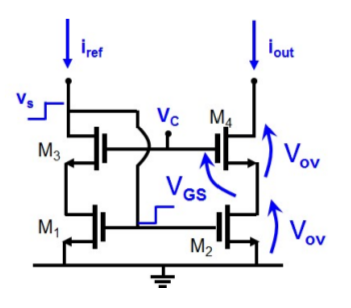
\includegraphics[width=0.35\textwidth]{mirrorload.png}\\
\raggedright

\subsection{p-mos dynamics}


\centering
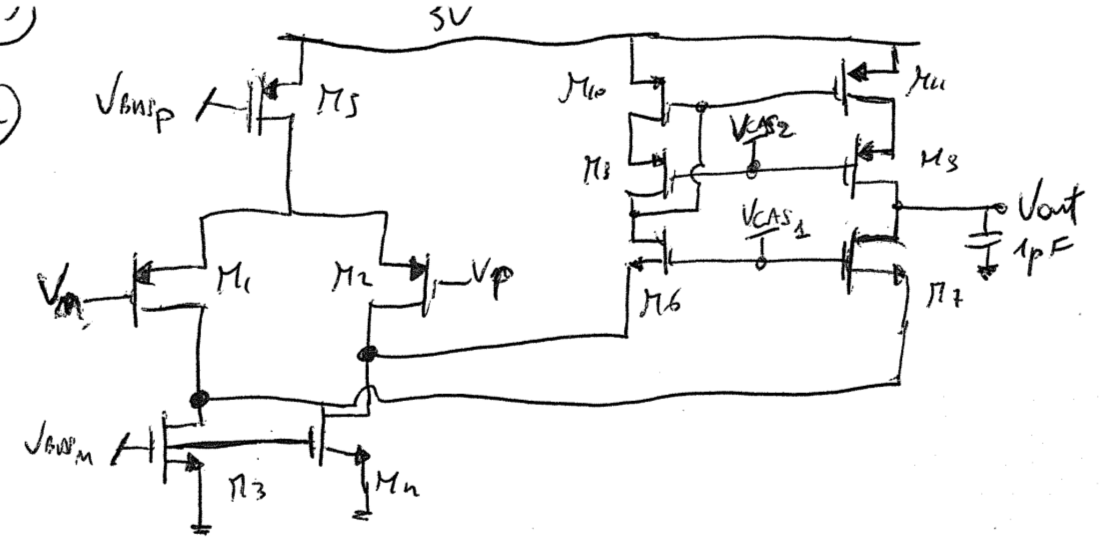
\includegraphics[width=0.5\textwidth]{pfcas.png}\\
\raggedright


TE 6 sept 2013\\

\subsection{Noise}
Cascode doesn't ifluence noise so we get
\begin{equation}
E_{wn}=\frac{8kT\gamma}{g_m^{in}}\left(1+\frac{g_m^{mirror\ high}}{g_m^{in}}+\frac{g_m^{g,current}}{g_m^{in}}   \right)
\end{equation}








{\it Remember to prevent the degradetion of the amplifier time response $I_G$ must be $>2I_1$}










